\documentclass[10pt, aspectratio=169]{beamer}
% hi
\usetheme{metropolis}
\metroset{block=fill}
\usepackage{appendixnumberbeamer}

\usepackage{booktabs}
\usepackage[scale=2]{ccicons}

\usepackage{siunitx}

\usepackage{xspace}
\newcommand{\themename}{\textbf{\textsc{metropolis}}\xspace}

\usepackage{amsmath}
\def\RR{\mathbb{R}}
\def\Pr{\mathrm{Pr}}

\usepackage{tikz}
\usetikzlibrary{positioning, arrows}
\usetikzlibrary{decorations.pathreplacing}
\usetikzlibrary{calc}
\usepackage{pgfplots}
\usepgfplotslibrary{dateplot}
\tikzset{
  font=\small,
  node distance=0.5cm and 0.2cm,
  bdata/.style={draw, rectangle, text width=2.2cm, align=center},
  sdata/.style={draw, rectangle, text width=1.75cm, align=center},
  bmodel/.style={rectangle, fill=mLightBrown, text width=4cm, align=center, rounded corners},
  smodel/.style={rectangle, fill=mLightBrown, text width=2.2cm, align=center, rounded corners},
  pred/.style={draw, rectangle, text width=1cm, align=center}
}

\usepackage[
  style=numeric,
  isbn=false,
  url=true
  ]{biblatex}
\addbibresource{lit.bib}

\usepackage{graphicx}
\usepackage{xcolor}
\usepackage{hyperref}

\definecolor{mDarkTeal}{HTML}{23373b}
\definecolor{mLightBrown}{HTML}{EB811B}
\definecolor{mDarkBrown}{HTML}{B85002}
\definecolor{mLightGreen}{HTML}{14B03D}

\title{Beating the International Prognostic Index for high-risk DLBCL patients}
\subtitle{Master thesis progress report}
\date{March 12, 2024}
\author{Lukas Geßl}
\institute{Chair of Statistical Bioinformatics, Regensburg University}
% \titlegraphic{\hfill
\includegraphics[height=1.5cm]{logo.jpeg}}

\begin{document}

\maketitle

\section{Set the arena}

\begin{frame}{DLBCL: a heterogeneous cancer with a homogeneous therapy}
  In practice, there is only one treatment regimen: immunochemotherapy with R-CHOP. 
  It cures two thirds of the patients.

  Cure rates among relapsed and refractory patients are low. Hence, we should not send 
  them to R-CHOP therapy in the first place, but into alternative treatments including 
  clinical trials.
  
  \pause
  We define \alert{high-risk} patients as those with a 
  \alert{progression-free survival (PFS) < 2 years}.

  \medskip
  \begin{block}{The goal of this thesis (and the MMML-Predict project) is ...}
    ... to develop a \alert{cost-efficent ($< \num{1500}$ euros) classifier filtering out 
    high-risk DLBCL patients} before an R-CHOP treatment begins or at least at an early 
    stage of it.
  \end{block}
\end{frame}

\begin{frame}{}
  Candidate input features for the new classifier are 
  \begin{itemize}
    \item clinical data (like the IPI, see next slide),
    \item transcriptomic (RNA-seq, signatures like LAMIS, ABC vs. GCB),
    \item proteomic signatures,
    \item somatic genetic factors (translocations like MYC),
  \end{itemize}
  all of which are measured \alert{at diagnosis}, as well \alert{dynamic} features like 
  \begin{itemize}
    \item the tumor burden according to a liquid biopsy after 2 and 4 cycles of R-CHOP. 
  \end{itemize}

\end{frame}

\begin{frame}{To beat: the International Prognostic Index (IPI) for non-Hodgkin's lymphoma}
  The IPI \autocite{ipi93} is a simple risk score ranging from 0 to 5 depending on how many of the following 
  \alert{clinical} questions for a patient one can answer with "yes": 

  \begin{itemize}
    \item Age > 60?
    \item Ann Arbor stage III or IV: is the cancer advanced?
    \item Serum LDH (lactacte dehydrogenase) level: higher than normal?
    \item Performance status: is the patient no longer ambulatory? 
    \item Number of extranodal sites (like bone marrow, liver, lung) involved: more than one?
  \end{itemize}

  \pause
  The lower the IPI, the better the patient's outlook: higher progression-free survival (PFS) and 
  overall survival (OS).
\end{frame}

\begin{frame}{The IPI is a 30-year old dinosaur}

  Yet, it's still state of the art in clinical practice when it comes to assessing a DLBCL 
  patient's risk  because it's \alert{simple}, \alert{cheap} and 
  \alert{robust} (after all, it's based on a rigorous statistical analysis and Cox regression).

  Still, just six values the IPI can attain mean it's very rough. In particular, it fails 
  to identify a clinically relevant high-risk group:

  \pause
  \begin{itemize}
    \item The cohort with IPI $= 5$ is \alert{too small} to get attention from clincians.
    \item The cohort with IPI $\geq 4$ \alert{lacks precision\footnote{Proportion of true 
      positives among all positives.} in identifying high-risk patients}: 16\% of patients have 
      an IPI $\geq 4$, but only 40\% of them are high-risk. This is too low to persuade 
      a clinician to change the treatment plan.
  \end{itemize}

\end{frame}

\begin{frame}{What does "beating the IPI" mean?}
  We need data to demonstrate the new classifier's superiority. MMML-Predict aims to enroll 300 DLBCL 
  patients (200 training, 100 test cohort). For my thesis, I need to use already existent data.

  \pause
  Beating the IPI means, on the test cohort the new classifier needs to 

  \begin{itemize}
    \item be \alert{more precise in identifying high-risk patients} than the IPI: the 95\% confidence interval (CI) 
    of the precision according to Clopper-Pearson  
    must not include 35\%\footnote{This is the  precision of IPI $\geq 4$ on pooled data from DSNHNL trials 
    ($\num{2721}$ samples).},
    \item yield \alert{two cohorts with significantly differing survival} (PFS): logrank-test p-value < 0.05.
  \end{itemize}

  \pause
  Calculations with the size of the test cohort ($n = 100$) suggest that a precision $\geq 50\%$ with a 
  prevalence\footnote{The rate of positive predictions.} $\geq 15\%$ is enough.
\end{frame}

\section{Meet the players}

\begin{frame}{\alert{Early} versus late integration}
  \begin{columns}
    \column{0.5\textwidth}
      \centering
      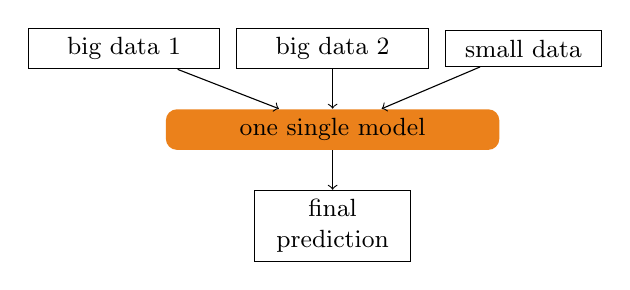
\begin{tikzpicture}
        \node[bdata] (bigdata1) {big data 1};
        \node[bdata, right=of bigdata1] (bigdata2) {big data 2};
        \node[sdata, right=of bigdata2] (smalldata) {small data};
        \node[bmodel, below=of bigdata2] (latemodel) {one single model};
        \node[sdata, below=of latemodel] (latepred) {final prediction};
        
        \draw[->] (bigdata1) -- (latemodel);
        \draw[->] (bigdata2) -- (latemodel);
        \draw[->] (smalldata) -- (latemodel);
        \draw[->] (latemodel) -- (latepred);
      \end{tikzpicture}
    \column{0.5\textwidth}
      \begin{itemize}
        \item Provide all data as input features to a single well-known model.
        \item Upside: easy to implement, one algorithm fits and picks the model 
          including a cross validation.
        \item Downside: data on vastly different scales may confuse the model and 
          its minimizer.
      \end{itemize}
  \end{columns}
\end{frame}

\begin{frame}{Early versus \alert{late} integration}
  \begin{columns}
    \column{0.5\textwidth}
      \centering
      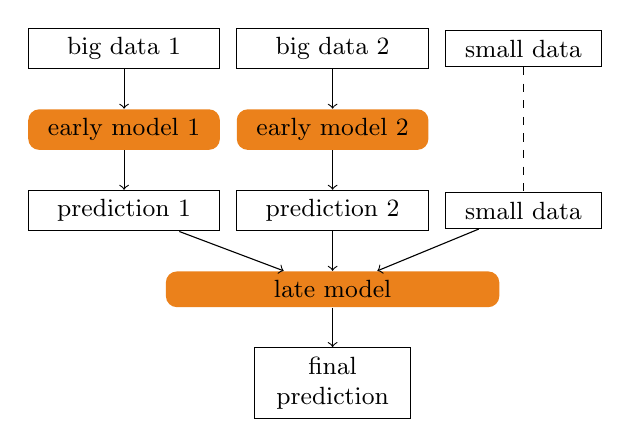
\begin{tikzpicture}  
        \node[bdata] (bigdata1) {big data 1};
        \node[bdata, right=of bigdata1] (bigdata2) {big data 2};
        \node[sdata, right=of bigdata2] (smalldata) {small data};
        \node[smodel, below=of bigdata1] (earlymodel1) {early model 1};
        \node[smodel, right=of earlymodel1] (earlymodel2) {early model 2};
        \node[bdata, below=of earlymodel1] (earlypred1) {prediction 1};
        \node[bdata, right=of earlypred1] (earlypred2) {prediction 2};
        \node[sdata, right=of earlypred2] (esmalldata) {small data};
        \node[bmodel, below=of earlypred2] (latemodel) {late model};
        \node[sdata, below=of latemodel] (latepred) {final prediction};
        
        \draw[->] (bigdata1) -- (earlymodel1);
        \draw[->] (earlymodel1) -- (earlypred1);
        \draw[->] (bigdata2) -- (earlymodel2);
        \draw[->] (earlymodel2) -- (earlypred2);
        \draw[dashed] (smalldata) -- (esmalldata);
        \draw[->] (earlypred1) -- (latemodel);
        \draw[->] (earlypred2) -- (latemodel);
        \draw[->] (esmalldata) -- (latemodel);
        \draw[->] (latemodel) -- (latepred);
      \end{tikzpicture}
    \column{0.5\textwidth}
      \begin{itemize}
        \item Early models deal with high-throughput data and its curses: curse 
          of high dimensionality, measurement errors.
        \item Upside: modularizes the model selection process, allows for very
          sophisticated late models.
        \item Downside: implementing the model selection process becomes more 
          complicated, how to deal with cross validation in the early models?
      \end{itemize}
  \end{columns}
\end{frame}

\begin{frame}{The key player for early-stage models: zeroSum}
  We feed high-troughput data into 

  \begin{itemize}
    \item \alert{Cox} proportional-hazards models and
    \item \alert{logistic} models,
  \end{itemize}

  with \alert{LASSO} regularization and the \alert{zero-sum} constraint. Both  
  aim to estimate the response $y_i$ of sample $i$ by a predictor $x_i \in \mathbb{R}^p$ via 
  \begin{align}
    y_i = f(\beta_0 + x_i^T \beta) + \varepsilon_i
  \end{align}
  for a link function $f: \mathbb{R} \to \mathbb{R}$, a vector of coefficients $(\beta_0, 
  \beta)$, and a residual $\varepsilon_i$.

  \pause
  The zero-sum constraint, $\sum_{j=1}^p \beta_j = 0$, enforces \alert{scale-invariance}, i.e., 
  the model output for $\alpha \cdot x_i$ ($\alpha > 0$) \textit{after taking the log} is the same 
  as for $x_i$.
\end{frame}

\begin{frame}{Wrap it all into a loss function}
  Training such a model comes down to minimizing a loss function of the form 
  \begin{align}
    \mathcal{L}_{X, y, \lambda, u, v, w}(\beta_0, \beta) = -\sum_{i=1}^n w_i 
    \ell_{X, y, \beta}(\tilde{y}_i, \beta_0 + x_i^T \beta) + \lambda \sum_{j=1}^p v_j |\beta_j| 
    \quad \text{subject to } \sum_{j=1}^p u_j \beta_j = 0
  \end{align}
  for hyperparameters 
  \begin{itemize}
    \item $\lambda > 0$, the LASSO penalty factor (tuned in a cross-validation),
    \item $u \in \RR^p_{\geq 0}$, the zero-sum weights (often $u = \mathbf{1}$),
    \item $v \in \RR^p_{\geq 0}$, the LASSO penalty weights (often $v = \mathbf{1}$), and
    \item $w \in \RR^n_{\geq 0}$, the sample weights (often $w = \frac{1}{n} \mathbf{1}$).
  \end{itemize}

  $\ell_{X, \tilde{y}, \beta}: \RR^2 \to \RR$ is some kind of model-dependent log likelihood. $\tilde{y}_i$ 
  is closely related to $y_i$ (if not the same), its nature again depends on the model.
\end{frame}

\begin{frame}{More on $\ell$ and $y_i$}
  In the \alert{Cox} model,
  \begin{itemize}
    \item $y_i$ is the \alert{relative hazard} of sample $i$: the higher it is, the earlier we 
      expect sample $i$ to face the event compared to the other samples.
    \item $\tilde{y}_i$ is the time to event.
    \item $\ell_{X, \tilde{y}, \beta}$ tries to enforce the correct ordering: $\beta_0 + x_i^T \beta$ 
      should be monotonic in $\tilde{y}_i$.
  \end{itemize}

  \pause
  In the \alert{logistic} model,
  \begin{itemize}
    \item we need to \alert{threshold the time to event} to get a \alert{binary response}: 
      $\tilde{y}_i = y_i = 1$ if the event happens before a certain time $T$, $0$ otherwise. 
      One can view \alert{$T$} as yet \alert{another hyperparameter}.
    \item $\ell_{X, \tilde{y}, \beta}$ forces $\beta_0 + \beta x_i^T$ to be high if 
      $\tilde{y}_i = 1$ and low else.
  \end{itemize}
\end{frame}

\begin{frame}{What this means for right-censoring}
  In reality, the data contains patients that dropped out of the study before the event could 
  occur (right-censoring).

  The Cox model, more precisely $\ell_{X, \tilde{y}, \beta}$, can take this information into 
  account.

  For the logistic model, however, we cannot use patients censored before $T$.
\end{frame}

\section{Train the players and select the best}

\begin{frame}{Train-test paradigm}
  \begin{columns}
    \column{.5\textwidth}
      \centering
      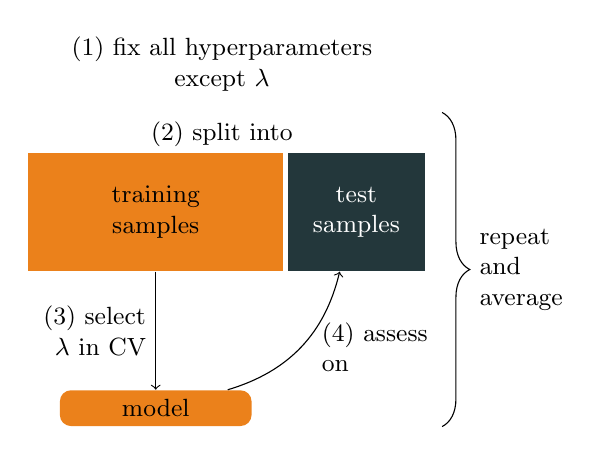
\begin{tikzpicture}[
        node distance=1cm and 0.05cm,
        trainn/.style={rectangle, text width=3cm, align=center, fill=mLightBrown, minimum height=1.5cm},
        testn/.style={rectangle, text width=1.5cm, align=center, fill=mDarkTeal, text=white, minimum height=1.5cm},  
        fixn/.style={rectangle, text width=4.7cm, align=center},
        splitn/.style={rectangle, text width=4.5cm, align=center}
        ]
        \node[trainn] (traindata) {training\\ samples};
        \node[testn, right=of traindata] (testdata) {test samples};
        \node[splitn, above=0.7cm of $(traindata)!0.33!(testdata)$] (split) {(2) split into};
        \node[fixn, above=0.15cm of split] (fixhyper) {(1) fix all hyperparameters\\ except $\lambda$};
        \node[smodel, below=1.5cm of traindata] (model) {model};
        
        \draw[->] (traindata) -- node[midway, left, align=right] {(3) select\\ $\lambda$ in CV} (model);
        \draw[->] (model) to[bend right] node[midway, right=4pt, align=left] {(4) assess\\ on} (testdata);

        \path let \p1 = (split.east) in \pgfextra{\xdef\bracex{\x1}};
        \path let \p1 = (split.north) in \pgfextra{\xdef\braceuy{\y1}};
        \path let \p1 = (model.south) in \pgfextra{\xdef\bracely{\y1}};
        \draw[decorate,decoration={brace,amplitude=10pt,mirror,raise=12pt}] 
          (\bracex, \bracely) -- (\bracex, \braceuy) node[midway, right=22pt, align=left] {repeat\\ and\\ average};
      \end{tikzpicture}
    \column{.5\textwidth}
      \alert{Hyperparameters} excluding $\lambda$ may be
      \begin{itemize}
        \item the model type,
        \item zero-sum weights, regularization weights, sample weights,
        \item the threshold $T$ for the logistic model\footnotemark{}.
      \end{itemize}
      We \alert{assess} the models
      \begin{itemize}
        \item with a scalar metric (like the ROC-AUC) to get a \alert{pre-selection},
        \item in scatter plots (like prevalence versus precision) to \alert{threshold the scores} 
          output by the pre-selected models.
      \end{itemize}
    \end{columns}
    \footnotetext{Similarly for the Cox model, we can right-censor samples with time to event $> T$ at $T$.}
\end{frame}

\begin{frame}{Software}
  \alert{zeroSum R package} \autocite{zerosumR} for fitting and cross-validating the logistic and Cox models. 
  It extends the glmnet package by the zero-sum constraint.

  \pause
  When integrating a model selected in a cross validation into another model I want to continue the cross 
  validation of the early model. zeroSum does not report enough details, so I added this functionality in 
  a \alert{fork zeroSumLI} \autocite{zerosumliR}.

  \pause
  Training and assessing a bunch of models on several data sets means a lot of administrative, repetitive 
  work. I automized and outsourced this part into an \alert{R package patroklos} \autocite{patroklos}.
\end{frame}

\section{Watch the game: the results}

\begin{frame}{The data}
  I trained models predicting progression-free survival $< 2$ years on data including bulk RNA-seq 
  taken from Schmitz et al. \autocite{schmitz18}. 
  \begin{columns}
    \column{.6\textwidth}
      \begin{itemize}
        \item It has $n = \num{229}$ patients with survival information, $p = \num{25066}$ genes.
        \item $\num{78}$ (34\%) of these are high risk.
        \item $\num{135}$ (59\%) are low risk. 
        \item $\num{16}$ (7\%) we cannot assign.
        \item All IPI features are available in pheno data.
        \item The IPI does a pretty good job on it, see Table \ref{fig:ipi-schmitz}.
      \end{itemize}
    \column{.4\textwidth}
      % latex table generated in R 4.3.2 by xtable 1.8-4 package
% Mon Feb 19 15:25:19 2024
\begin{table}[ht]
\centering
\begin{tabular}{rrr}
  \hline
IPI $\geq$ & prevalence & precision \\ 
  \hline
  5 & 0.01 & 1.00 \\ 
    4 & 0.13 & 0.65 \\ 
    3 & 0.35 & 0.55 \\ 
    2 & 0.59 & 0.48 \\ 
    1 & 0.85 & 0.41 \\ 
    0 & 1.00 & 0.37 \\ 
   \hline
\end{tabular}
\caption{Classifying PFS < 2 years on \autocite{schmitz18}.} 
\label{fig:ipi-schmitz}
\end{table}

  \end{columns}
\end{frame}

\begin{frame}{The line-up: the models tried out}
  \begin{table}[ht]
    \centering
    \begin{tabular}{p{.20\textwidth}p{.73\textwidth}}
        \hline
        hyperparamter & choices \\ 
        \hline
        model family & Cox, logistic regression. \\
        input data & Gene expression only; gene expression with early integrated IPI: 
            as one continuous variable ("with ipi cont") or five binary variables ("with disc ipi feat"). \\ 
        zero-sum weights & $u = 0$; $u_i = 1$ for gene-expression features, 
            else $u_i = 1$ ("zerosum"). \\
        LASSO weights & Standardization, i.e., $v_i$ is the standard deviation of feature $i$ ("std"); 
            $v_i = 1$ for gene-expression features, else $0$. \\
        sample weights & $w = \mathbf{1}/n$. \\
        $T$ & $1, 1.25, 1.5, \ldots, 2.5$; additionally $\infty$ for Cox. \\
       \hline
    \end{tabular}
    \caption{Terms in quotation marks are used in model names on the following slides.}
    \label{fig:hyperpara-schmitz}
    \end{table}
\end{frame}

\begin{frame}{Pre-selection via ROC-AUC}
  \begin{columns}
    \column{.5\textwidth}
    {
      \small
      % latex table generated in R 4.3.2 by xtable 1.8-4 package
% Mon Feb 19 15:25:19 2024
\begin{table}[ht]
\centering
\begin{tabular}{rlrr}
  \hline
rank & model & $T$ & AUC \\ 
  \hline
   1 & logistic & 1.75 & 0.770 \\ 
     2 & logistic zerosum & 1.75 & 0.769 \\ 
     3 & cox & 1.75 & 0.762 \\ 
     4 & cox zerosum & 1.75 & 0.761 \\ 
     5 & cox & 2 & 0.755 \\ 
     6 & logistic zerosum & 1.5 & 0.755 \\ 
     7 & cox zerosum & 1.5 & 0.752 \\ 
     8 & cox & 1.5 & 0.750 \\ 
     9 & cox & Inf & 0.749 \\ 
    10 & cox zerosum & Inf & 0.748 \\ 
   \hline
\end{tabular}
\caption{Split into train and test cohort, train a model on train cohort, calculate ROC-AUC
        on test cohort. Repeat this 15 times and average.} 
\label{fig:top-auc-schmitz}
\end{table}

    }
    \column{.5\textwidth}
      What does this mean for choosing the hyperparameters?
      \begin{itemize}
        \item Logistic versus Cox regression not that important.
        \item With zero-sum constraint usually a bit worse than without.
        \item Choose $T = 1.75$.
        \item Early integration and standardization disappoint.
      \end{itemize}
  \end{columns}
\end{frame}

\begin{frame}{Is this enough to meet our initially stated goals?}
  \begin{figure}[h]
    \centering
    \includegraphics[width=.9\textwidth]{figs/precision.jpeg}
  \end{figure}
\end{frame}

\begin{frame}{Is this enough to meet our initially stated goals?}
  \begin{figure}[h]
    \centering
    \includegraphics[width=.9\textwidth]{figs/precision_ci.jpeg}
  \end{figure}
\end{frame}

\begin{frame}{Is this enough to meet our initially stated goals?}
  \begin{figure}[h]
    \centering
    \includegraphics[width=.9\textwidth]{figs/logrank.jpeg}
  \end{figure}
\end{frame}

\section{What comes next?}

\begin{frame}{}
  \textbf{On the data front}, I want to  
  \begin{itemize}
    \item do the afore-mentioned on a \alert{bigger ($n = 624 \gg 229$) data set} by Reddy 
      et al. \autocite{reddy17}. 
    \item Downside: only overall, no progression-free survival included (fine 
      for this thesis, less helpful for MMML-Predict).
  \end{itemize}

  \pause
  \textbf{On the methods front}, I want to 
  \begin{itemize}
    \item try to get \alert{early integration} with zeroSum working,
    \item use sample weights $w \neq \frac{1}{n} \mathbf{1}$ to give less weight to patients with 
      a PFS close to 2 years in the loss,
    \item implement \alert{late integration}: with, e.g., linear regression, random forest as second-
      stage models,
    \item integrate more features.
  \end{itemize}
\end{frame}

\begin{frame}[standout]
  Thank you for your attention! \par Questions?
\end{frame}

\appendix

\begin{frame}[allowframebreaks]{References}
  \printbibliography
\end{frame}

\end{document}